\section{Empirical Findings}
\label{sec:experiments}

\subsection{Setup}

We evaluate 12 complete P1--P4 model runs on the 763-task VEH benchmark: gpt-5.4, \texttt{qwen3.6-plus}, deepseek-v3, claude-4.6-sonnet, qwen3-max, deepseek-r1, gemini-3.1-pro-preview, \texttt{o4-mini}, \texttt{llama-3.3-70b}, deepseek-v4-pro, mimo-v2.5-pro, and hunyuan-hy3-preview. Here \(n=12\) denotes model-level observations with all four probes complete, not a development split. The headline metrics are P1-Composite, P2 final feasible power ratio, P3-Success, and P4 full-bank Kendall Tau. Calibration references, split-resolved tables, uncertainty intervals, metric definitions, prompt templates, and the run-mode audit are in the appendix.

\subsection{Stage Dissociation: Engineering Ability Is Not One Scalar}

\begin{table*}[t]
\caption{Twelve-model P1--P4 headline results on the 763-task VEH benchmark. \texttt{Think} marks whether this run used reasoning/thinking mode; detailed run-mode evidence is in Appendix Table~\ref{tab:appendix_reasoning_grouping}.}
\label{tab:main_results}
\centering
\scriptsize
\setlength{\tabcolsep}{4pt}
\renewcommand{\arraystretch}{1.08}
\begin{tabular}{llcccc}
\toprule
Model & Think & P1 Comp. & P2 Ratio & P3 Succ. & P4 Tau \\
\midrule
qwen3-max & No & \textbf{0.574} & 0.1955 & 30.1 & 0.835 \\
gemini-3.1-pro-preview & Yes & 0.549 & \textbf{0.3904} & 37.2 & 0.824 \\
\texttt{o4-mini} & Yes & 0.518 & 0.1551 & 26.3 & 0.780 \\
deepseek-r1 & Yes & 0.504 & 0.2413 & 42.9 & 0.833 \\
gpt-5.4 & No & 0.428 & 0.1329 & 42.3 & \textbf{0.887} \\
hunyuan-hy3-preview & Yes & 0.425 & 0.1609 & \textbf{47.4} & 0.839 \\
deepseek-v3 & No & 0.369 & 0.1565 & 35.3 & 0.860 \\
\texttt{llama-3.3-70b} & No & 0.361 & 0.1197 & 3.2 & 0.714 \\
mimo-v2.5-pro & No & 0.317 & 0.1073 & 45.5 & 0.843 \\
\texttt{qwen3.6-plus} & No & 0.306 & 0.2063 & 27.6 & 0.877 \\
deepseek-v4-pro & No & 0.306 & 0.1294 & 28.8 & 0.794 \\
claude-4.6-sonnet & No & 0.207 & 0.2394 & 16.0 & 0.840 \\
\bottomrule
\end{tabular}
\end{table*}

Table~\ref{tab:main_results} is the central result. P1 is P1-Composite, P2 is final feasible power ratio, P3 is recovery success, and P4 is full-bank Kendall Tau; detailed run-mode evidence is in Appendix Table~\ref{tab:appendix_reasoning_grouping}. No model leads more than one headline stage: qwen3-max leads P1, gemini-3.1-pro-preview leads P2, hunyuan-hy3-preview leads P3, and gpt-5.4 leads P4. The strongest reversal is gemini-3.1-pro-preview versus gpt-5.4. gemini-3.1-pro-preview is the best feasible-set seeker in P2 but weak on P4 ranking; gpt-5.4 is the best policy-conditioned ranker but weak on P2 search. If engineering ability were one scalar, this pattern should be rare.

The within-stage diagnostics sharpen the same point. \textbf{P1 finding:} credible triage is not raw accuracy; qwen3-max wins the composite through balanced action discipline, while models with acceptable raw accuracy collapse once missing-information and infeasibility discipline are scored. \textbf{P2 finding:} start is not finish; gemini-3.1-pro-preview is not the best first-step model, but wins through sustained feasibility-preserving closure. \textbf{P3 finding:} escape is not recovery; gemini-3.1-pro-preview and claude-4.6-sonnet escape traps frequently but have very different cascade and final-success behavior. \textbf{P4 finding:} ranking is not one skill; full-order structure, exact endpoint agreement, and policy-active ranking separate. The full per-probe tables are in Appendix Tables~\ref{tab:appendix_p1_full}--\ref{tab:appendix_p4_full}.

\subsection{Response-Control Profiles: Why Dissociation Happens}

We next quantify response-control profiles directly from logs. The extractor uses P1 action distributions and false-action rates; P2 edit deltas, feasibility preservation, directed repair, and objective traces; P2/P3 verifier-feedback reduction consistency; P3 escape, cascade, dead-budget, and recovery-quality signals; and P4 full-ranking, BARS, exact-match, policy-sensitive-pair, parse, and Pareto diagnostics. The complete 12-model profile table is in Appendix Table~\ref{tab:profile_quantification}.

The intended diagonal relations are strong associations: action prior tracks P1-Composite (Spearman \(\rho=0.972\)), edit style tracks P2 ratio (\(\rho=0.839\)), and preference execution tracks P4 BARS (\(\rho=0.769\)) and full Tau (\(\rho=0.762\)). State trust is more structured: it does not monotonically track P3-Success because P3 separates escape, cascade, and conversion to feasibility, but it is negatively correlated with P2 ratio (\(\rho=-0.39\)) and P4 BARS (\(\rho=-0.55\)). A prior associated with strength at one boundary can therefore be associated with weakness at another.

\subsection{Ruling Out the Reasoning/Newness Explanation}

\begin{table*}[t]
\caption{Thinking mode versus response-control profile fit. Thinking-on runs help P3 on average but do not explain P1, P2, or P4 leaders; profile indicators localize the boundary-specific mechanism.}
\label{tab:reasoning_vs_profile}
\centering
\small
\setlength{\tabcolsep}{4.5pt}
\renewcommand{\arraystretch}{1.12}
\begin{tabular}{lccp{70mm}}
\toprule
Stage & Think & No-think & Profile-based interpretation \\
\midrule
P1 Composite & 0.499 & 0.359 & thinking-on runs are still not sufficient for triage; qwen3-max leads under a no-think provider-default call because action discipline is the measured dimension \\
P2 headline & 0.237 & 0.161 & gemini-3.1-pro-preview drives the think mean, but the operative boundary fit is bounded local edit style plus feedback obedience \\
P3 Success (\%) & 38.5 & 28.6 & largest group gap; corrupted-state recovery is where state skepticism and explicit replanning are most useful \\
P4 Full Tau & 0.819 & 0.831 & reversal; thinking mode does not guarantee policy-conditioned evaluator discipline \\
\bottomrule
\end{tabular}
\end{table*}

Table~\ref{tab:reasoning_vs_profile} rules out the shallow reading that DiagBench is only a reasoning-model leaderboard. Thinking-on runs help the corrupted-state boundary on average, but they do not determine the P1, P2, or P4 frontier. The same is true for recency: deepseek-v4-pro does not monotonically dominate deepseek-v3 or deepseek-r1. A more diagnostic account is boundary fit: P2 rewards bounded repair, P3 rewards state skepticism, and P4 rewards evaluator-role discipline.

\subsection{Mechanism Evidence: Four Validity Challenges, Four Responses}

We test four alternative explanations with matched audits: repair versus corrupted-state recovery, selection versus generation, LLM repair versus generic optimization, and structural profile mismatch versus prompt artifact. Each audit changes one part of the evaluation setup while keeping the relevant task boundary fixed.

\paragraph{Corrupted recovery is not clean repair.}
If P3 failure were only weak repair, replacing raw trajectory history with a verifier-authored state summary should not help systematically. If failure reflects corrupted-state entrapment, the intervention should reduce cascade and improve recovery. Figure~\ref{fig:mechanism_evidence} shows the expected pattern: \texttt{state\_summary} raises model-mean recovery from 50.0\% to 63.2\% and lowers cascade from 28.1\% to 9.5\%. Full numeric deltas and confidence intervals are in Appendix Table~\ref{tab:appendix_p3_intervention_delta_ci}.

\begin{figure*}[t]
\centering
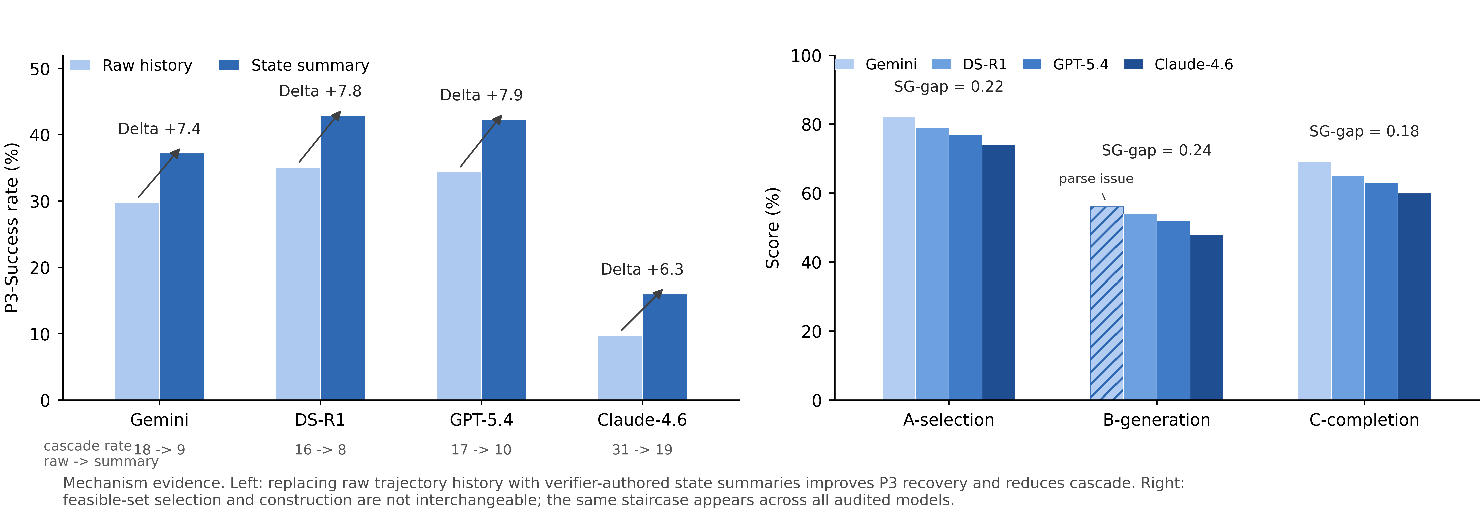
\includegraphics[width=\linewidth,trim=0 28bp 0 0,clip]{figures/main/selection_generation_gap.pdf}
\vspace{-5mm}
\caption{P3 intervention mechanism evidence. (A) Replacing raw trajectory history with a verifier-authored state summary improves recovery success for most models. (B) The same intervention reduces harmful cascade, showing that P3 is a corrupted-state boundary rather than ordinary clean repair. Full numeric results appear in Appendix Table~\ref{tab:appendix_p3_intervention_delta_ci}.}
\label{fig:mechanism_evidence}
\vspace{-3mm}
\end{figure*}

\paragraph{Selection is not generation.}
If P2 and P4 measured the same ability, selecting a feasible design should resemble generating it. The isomorphic audit holds the underlying feasible design fixed and changes only the model's role; it shows a 26--61 point gap between A-selection and B-generation. The gap is mostly capability rather than parsing for gpt-5.4, claude-4.6-sonnet, and \texttt{qwen3.6-plus}, supporting the claim that evaluative and generative priors are distinct. Full numeric results are in Appendix~\ref{sec:appendix_isomorphic}.

\paragraph{Repair is not generic optimization.}
If P2 reduced to numerical optimization, CMA-ES~\citep{hansen2023cma} should match LLM repair under the same 6-query oracle budget. It reaches 0.269 final feasible rate and 0.099 mean power ratio, below every frontier LLM; even at 40 queries it remains below gemini-3.1-pro-preview's P2 ratio. Full results appear in Appendix~\ref{sec:appendix_cmaes}, and the main conclusion is that P2 is not only an optimizer ceiling effect.

\paragraph{Profiles are not prompt artifacts.}
If the behavioral fingerprints above were shallow prompt artifacts, boundary-specific targeted prompts should repair known deficits. We test this with a pre-registered four-cell controlled-prompt experiment comparing default, neutral, targeted, wrong-boundary, and where applicable stacked prompts.

\begin{table*}[t]
\caption{Pre-registered controlled-prompt audit. Each cell reports the primary endpoint under the frozen prompt conditions; S+ denotes state-summary-plus for C2 only. Confidence intervals, secondary metrics, and parse rates are in Appendix~\ref{sec:tier3_full}.}
\label{tab:tier3_main}
\centering
\scriptsize
\setlength{\tabcolsep}{4pt}
\renewcommand{\arraystretch}{1.08}
\begin{tabularx}{\textwidth}{p{24mm}p{31mm}cccccY}
\toprule
Cell / endpoint & Model-stage & Default & Neutral & Targeted & Wrong & S+ & Readout \\
\midrule
C1 / P2 feasibility & gpt-5.4 & 0.150 & 0.175 & 0.150 & 0.075 & -- & targeted does not beat neutral \\
C2 / P3 success & claude-4.6-sonnet & 0.167 & \textbf{0.389} & 0.194 & 0.222 & 0.222 & neutral structure helps most \\
C3 / P4 Kendall $\tau$ & gemini-3.1-pro-preview & 0.692 & 0.692 & \textbf{0.708} & 0.700 & -- & one-task targeted gain \\
C4 / P1 accuracy & claude-4.6-sonnet & \textbf{0.650} & 0.617 & 0.567 & 0.633 & -- & targeted hurts format stability \\
C4 / P1 accuracy & gpt-5.4 & 0.433 & 0.400 & \textbf{0.467} & 0.400 & -- & small model-specific gain \\
\bottomrule
\end{tabularx}
\end{table*}

Table~\ref{tab:tier3_main} shows that targeted prompts do not consistently beat neutral structure. The strongest signal, claude-4.6-sonnet P3, reverses against the targeted prompt: neutral improves success most, while targeted and state-summary-plus remain low. This is consistent with durable prior-boundary mismatch rather than a signal that disappears under prompt rewriting; full condition-level results are in Appendix~\ref{sec:tier3_full}.

\subsection{Cross-Domain Construct Validity}

The mechanism audits address VEH-specific alternatives. The remaining question is whether the P1--P4 scaffold transfers when the physics changes. We instantiate a final circuit-design audit spanning closed-form RC filters, loaded dividers, LED current limiters, op-amp amplifiers, and linear regulators. It is not a circuit benchmark; it is a construct-validity check with a different oracle, different constraints, and different trap geometry.

\begin{table*}[t]
\caption{Circuit audit headline results. P1 is reported as P1-Composite; P2b is the final feasible objective score.}
\label{tab:circuit_pilot_headline}
\centering
\scriptsize
\setlength{\tabcolsep}{4pt}
\renewcommand{\arraystretch}{1.08}
\begin{tabular}{lccccccc}
\toprule
Model & P1 Comp. & P2 Feas. & P2b & P3 Succ. & P3 Casc. & P4 Tau & P4 BARS \\
\midrule
qwen3-max       & 0.971 & 0.906 & 0.494 & 0.778 & 0.471 & 0.608 & 0.710 \\
gemini-3.1-pro-preview  & \textbf{0.974} & \textbf{1.000} & \textbf{0.662} & \textbf{1.000} & \textbf{0.000} & 0.475 & 0.625 \\
gpt-5.4         & 0.923 & 0.875 & 0.457 & 0.778 & 0.176 & \textbf{0.625} & \textbf{0.722} \\
deepseek-r1     & \textbf{0.974} & 0.969 & 0.594 & 0.722 & \textbf{0.000} & 0.542 & 0.661 \\
hunyuan-hy3-preview     & 0.944 & 0.938 & 0.512 & 0.778 & 0.062 & 0.492 & 0.614 \\
claude-4.6-sonnet      & 0.932 & 0.906 & 0.487 & \textbf{1.000} & \textbf{0.000} & 0.608 & 0.707 \\
\midrule
Stage spread & 0.051 & 0.125 & 0.205 & 0.278 & 0.471 & 0.150 & 0.108 \\
\bottomrule
\end{tabular}
\end{table*}

Table~\ref{tab:circuit_pilot_headline} reproduces the main signature after replacing only P1/P2. No model dominates: gemini-3.1-pro-preview and deepseek-r1 tie the P1-Composite point estimate, gemini-3.1-pro-preview leads P2b, gemini-3.1-pro-preview and claude-4.6-sonnet retain the original P3 success lead, and gpt-5.4 retains the original P4 lead. The gpt-5.4 P4-over-P1/P2 reversal and gemini-3.1-pro-preview P2-over-P4 reversal both remain. The framework transfers; the rankings do not, which is what boundary-specific diagnosis predicts.
